\documentclass[xcolor=x11names,dvipsnames,compress]{beamer}

%% General document %%%%%%%%%%%%%%%%%%%%%%%%%%%%%%%%%%
\usepackage[default]{lato}
\usepackage{setspace}
\usepackage[T1]{fontenc}
\usepackage{graphicx}
\usepackage{amsmath}
\usepackage{amssymb}
\usepackage{amsfonts}
\usepackage{amssymb}
\usepackage{relsize}
\usepackage{multirow}
\usepackage{bm}
\usepackage{tikz}
\usepackage{epsfig}
\usepackage{epstopdf} 
\usepackage{float}
\usepackage{subfig}

\usetikzlibrary{decorations.fractals}
%%%%%%%%%%%%%%%%%%%%%%%%%%%%%%%%%%%%%%%%%%%%%%%%%%%%%%
\pdfmapfile{+lato.map}

%% Beamer Layout %%%%%%%%%%%%%%%%%%%%%%%%%%%%%%%%%%
\useoutertheme[subsection=false,shadow]{miniframes}
\useinnertheme{default}
%\usefonttheme{lato}
%\usepackage{palatino}

\setbeamerfont{title like}{shape=\scshape}
\setbeamerfont{frametitle}{shape=\scshape}

\setbeamercolor*{lower separation line head}{bg=DeepSkyBlue4} 
\setbeamercolor*{normal text}{fg=black,bg=white} 
\setbeamercolor*{alerted text}{fg=red} 
\setbeamercolor*{example text}{fg=black} 
\setbeamercolor*{structure}{fg=black} 
 
\setbeamercolor*{palette tertiary}{fg=black,bg=black!10} 
\setbeamercolor*{palette quaternary}{fg=black,bg=black!10} 

\renewcommand{\(}{\begin{columns}}
\renewcommand{\)}{\end{columns}}
\newcommand{\<}[1]{\begin{column}{#1}}
\renewcommand{\>}{\end{column}}
%%%%%%%%%%%%%%%%%%%%%%%%%%%%%%%%%%%%%%%%%%%%%%%%%%

%%%%%%%%%%%%%%%%%%%%%%%%%%%%%%%%%%%%%%%%%%%%%%%%%%%%%%%%%%%%%%%%%%%%%%%%%%%%%%%%
%%%% Some math symbols used in the text
%%%%%%%%%%%%%%%%%%%%%%%%%%%%%%%%%%%%%%%%%%%%%%%%%%%%%%%%%%%%%%%%%%%%%%%%%%%%%%%%
% Format 
\graphicspath{ {./gfx/} }

\addtobeamertemplate{navigation symbols}{}{%
    \usebeamerfont{footline}%
    \usebeamercolor[fg]{footline}%
    \hspace{1em}%
    \insertframenumber/\inserttotalframenumber
}

\begin{document}


%%%%%%%%%%%%%%%%%%%%%%%%%%%%%%%%%%%%%%%%%%%%%%%%%%%%%%
%%%%%%%%%%%%%%%%%%%%%%%%%%%%%%%%%%%%%%%%%%%%%%%%%%%%%%
\section{\scshape Introduction}
\begin{frame}
%\vspace{-2cm}
\title{A Biologically Inspired Model for Coding Sensorimotor Experience Leading to the Development of Pointing Behaviour in a Humanoid Robot}
\subtitle{Master's Thesis}
\author{
	Ivana Kaji\'c\\
	Bernstein Center for Computational Neuroscience Berlin, Germany \\
	\includegraphics[scale=0.2]{babies.jpg}
}
\date{}
\titlepage
\end{frame}


%%%%%%%%%%%%%%%%%%%%%%%%%%%%%%%%%%%%%%%%%%%%%%%%%%%%%%
%%%%%%%%%%%%%%%%%%%%%%%%%%%%%%%%%%%%%%%%%%%%%%%%%%%%%%
\subsection{\scshape Introduction}
\begin{frame}{What?}

\textcolor{Fuchsia}{A Biologically Inspired Model} for \textcolor{MidnightBlue}{Coding Sensorimotor Experience Leading to the Development of Pointing Behaviour} in a \textcolor{Emerald}{Humanoid Robot}


 \begin{itemize} 
      \item \textcolor{Fuchsia}{A Biologically Inspired Model}
      \begin{itemize}
      \item Neural networks and Hebbian learning
      \end{itemize}
     \item \textcolor{MidnightBlue}{Sensorimotor Experience Leading to the Development of Pointing Behaviour}
     \begin{itemize}
      \item We address questions from the developmental psychology
     \end{itemize}
     \item \textcolor{Emerald}{Humanoid Robot}
     \begin{itemize}
      \item We use a humanoid robot (Nao) that has similar physical dimensions as a human child
     \end{itemize}
 \end{itemize}
\end{frame}

%%%%%%%%%%%%%%%%%%%%%%%%%%%%%%%%%%%%%%%%%%%%%%%%%%%%%%
%%%%%%%%%%%%%%%%%%%%%%%%%%%%%%%%%%%%%%%%%%%%%%%%%%%%%%
\subsection{\scshape Introduction}
\begin{frame}[noframenumbering]
\Large Brain, Body and Behaviour
\end{frame}

%%%%%%%%%%%%%%%%%%%%%%%%%%%%%%%%%%%%%%%%%%%%%%%%%%%%%%
%%%%%%%%%%%%%%%%%%%%%%%%%%%%%%%%%%%%%%%%%%%%%%%%%%%%%%
\subsection{\scshape Introduction}
\begin{frame}{Behaviorism}
\begin{itemize}
 \item An approach to psychology that aims to explain the behaviour through experiments with animals and humans
 \item Concerned with observable consequences, not the internal processes
 \begin{figure}
\includegraphics[height=5cm]{pavlov.png}  
 \end{figure}
\end{itemize}
\end{frame}

%%%%%%%%%%%%%%%%%%%%%%%%%%%%%%%%%%%%%%%%%%%%%%%%%%%%%%
%%%%%%%%%%%%%%%%%%%%%%%%%%%%%%%%%%%%%%%%%%%%%%%%%%%%%%
\subsection{\scshape Introduction}
\begin{frame}{Cognitivism}
\begin{itemize}
 \item Explain the human behaviour in terms of underlying cognitive processes
 \item Gained popularity in artifical intelligence
 \begin{figure}
\includegraphics[height=4cm]{chess.png}  
 \end{figure}
\end{itemize}
\end{frame}

%%%%%%%%%%%%%%%%%%%%%%%%%%%%%%%%%%%%%%%%%%%%%%%%%%%%%%
%%%%%%%%%%%%%%%%%%%%%%%%%%%%%%%%%%%%%%%%%%%%%%%%%%%%%%
\subsection{\scshape Introduction}
\begin{frame}{But...}
\begin{itemize}
 \item The majority of artificial intelligence algorithms inspired by cognitivist theories were focusing on problem-solving skills 
    \begin{itemize}
     \item Unable to reproduce the complex spectrum of human behaviour (e.g.: perception, learning, emotions)
    \end{itemize}
 \item Post-cognitivism: the role of embodiment and neural processing 
 \begin{figure}
\includegraphics[height=4cm]{child-bike.png} 
\hspace{1cm}
\includegraphics[height=4cm]{neurons.png}  
 \end{figure}
\end{itemize}
\end{frame}

\section{\scshape The Task}
\begin{frame}[noframenumbering]
\Large The Task
\end{frame}


%%%%%%%%%%%%%%%%%%%%%%%%%%%%%%%%%%%%%%%%%%%%%%%%%%%%%%
%%%%%%%%%%%%%%%%%%%%%%%%%%%%%%%%%%%%%%%%%%%%%%%%%%%%%%
\subsection{\scshape The Task}
\begin{frame}{The goal of this thesis}
\begin{itemize}
 \item Simulate sensorimotor learning leading to the development of attentional mechanisms
 \begin{itemize}
  \item Robot simulates the sensory experience of a young child
  \item Learning inspired by the human behaviour: body babbling  
 \end{itemize}
 \item Develop a model of sensorimotor learning based on neural networks 
 \begin{itemize}
  \item Use self-organising maps and associate them using a Hebbian learning paradigm
 \end{itemize}
\end{itemize}
\end{frame}

\subsection{\scshape The Task}
\begin{frame}{Motivation}
 
  \begin{figure}[h!]  
  \centering
  \includegraphics[height=4cm]{girl1.png}
  \end{figure}  
  
  \begin{itemize}
  \item \textbf{Joint attention} is an important part of the development in infancy and \textbf{pointing} is one of the mechanisms used for attention manipulation
  \end{itemize}
\end{frame}

%%%%%%%%%%%%%%%%%%%%%%%%%%%%%%%%%%%%%%%%%%%%%%%%%%%%%%
%%%%%%%%%%%%%%%%%%%%%%%%%%%%%%%%%%%%%%%%%%%%%%%%%%%%%%
\subsection{\scshape The Task}
\begin{frame}{Related Work}
  \begin{itemize}
   \item  Sensorimotor learning and simulation of experience following the theories on the human development \cite{Schillaci}
  \end{itemize}
    \begin{figure}
    \centering
      \includegraphics[height=6cm]{experiments_note.png}
    \end{figure}
  
\end{frame}


\subsection{\scshape The Task}
\begin{frame}{Related work}
\begin{itemize}  
 \item Structured association of multiple SOMs has been adopted for mapping different modalities in Epigenetic Robotics Architecture \cite{Morse2010}
\end{itemize}
    \begin{figure}
    \centering
      \includegraphics[height=4cm]{era.png}
    \end{figure}
\end{frame}
%%%%%%%%%%%%%%%%%%%%%%%%%%%%%%%%%%%%%%%%%%%%%%%%%%%%%%
%%%%%%%%%%%%%%%%%%%%%%%%%%%%%%%%%%%%%%%%%%%%%%%%%%%%%%
\subsection{\scshape The Task}
\begin{frame}{Motor Babbling}
  \begin{itemize}
  \item Self-exploration strategy employed by infants to learn internal mappings of body postures
  \item Implemented on a humanoid robot using a random walk strategy
    \begin{itemize}
    \item The robot moved its left arm randomly - hands and joint positions were stored (cca. 40 min)
    \item Hand was tagged with a marker    
    \end{itemize}    
  \end{itemize}
 

    \begin{figure}   
  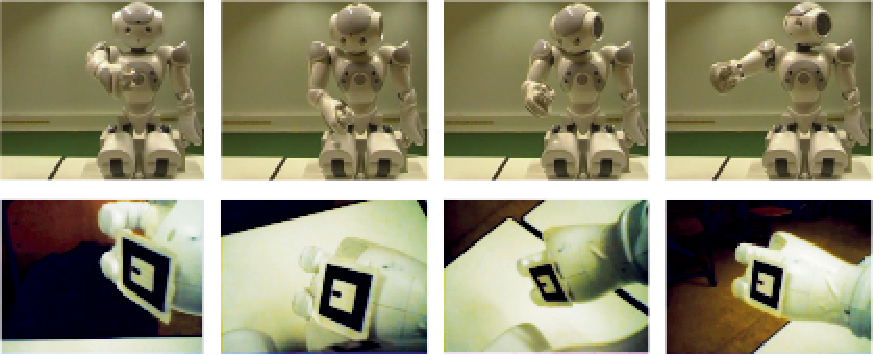
\includegraphics[height=3cm]{sequence.pdf}
  \end{figure}

\end{frame}


%%%%%%%%%%%%%%%%%%%%%%%%%%%%%%%%%%%%%%%%%%%%%%%%%%%%%%

\subsection{\scshape The Task}
\begin{frame}{Realisation}
  \begin{enumerate}
   \item Collect data in the random motor babbling experiment
   \begin{itemize}
    \item $74,143$ 7D data points (3D hand coordinates, 4D elbow and shoulder coordinates)
   \end{itemize}
   \item Train the SOM-based model on the data from the step 1.
    \begin{itemize}
     \item 2 different models: $5\times5$ and $15\times15$ model
    \end{itemize}
   \item Implement both models on the humanoid robot
   \item Run the experiment and use the model to determine arm positions
    \begin{itemize}
    \item A human subject holding an object tagged with a marker
    \end{itemize}    
  \end{enumerate}
\end{frame}


%%%%%%%%%%%%%%%%%%%%%%%%%%%%%%%%%%%%%%%%%%%%%%%%%%%%%%

%%%%%%%%%%%%%%%%%%%%%%%%%%%%%%%%%%%%%%%%%%%%%%%%%%%%%%
%%%%%%%%%%%%%%%%%%%%%%%%%%%%%%%%%%%%%%%%%%%%%%%%%%%%%%
\section{\scshape The Model}
\begin{frame}[noframenumbering]
\Large The Model
\end{frame}

\subsection{\scshape The Model}
\begin{frame}{The Model}
\begin{itemize}
\item Two 2D SOMs connected with Hebbian weights
  \begin{itemize}
   \item We analyse two different models with a different number of neurons: $5\times5$ (25 neurons in each map) model and $15\times15$ model (225 neurons in each map)
  \end{itemize}
  \begin{figure}
  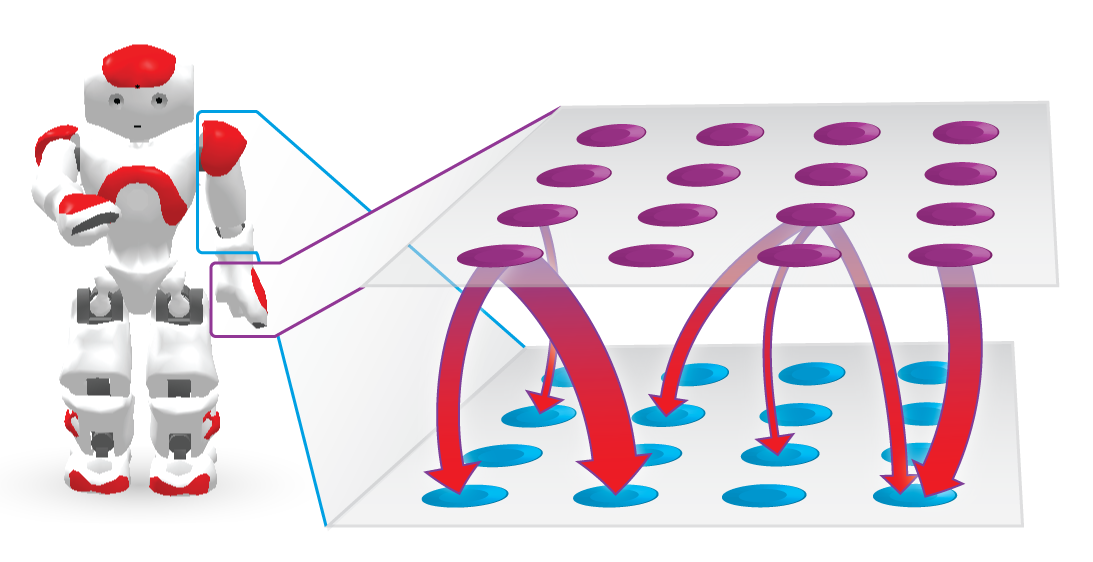
\includegraphics[width=0.8\textwidth]{model.png}
  \end{figure}
\end{itemize}
\end{frame}

\subsection{\scshape The Model}
\begin{frame}{Motivation for the model}
\begin{itemize}
\item Biologically inspired by self-organisation observed in the brain 
	\begin{itemize}
	\item Orientation maps in V1, somatotopic maps, tonotopic organisation of the auditory cortex
  	\end{itemize}
\begin{figure}
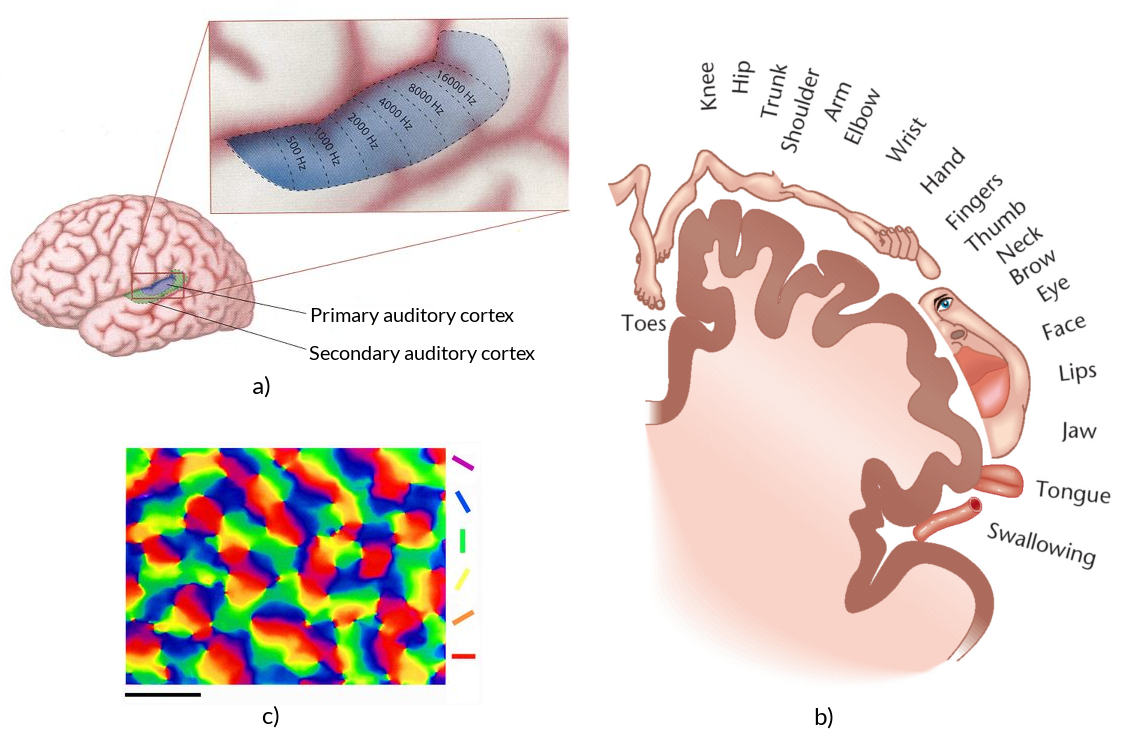
\includegraphics[height=4cm]{maps}
\end{figure}

\end{itemize}
\end{frame}



%%%%%%%%%%%%%%%%%%%%%%%%%%%%%%%%%%%%%%%%%%%%%%%%%%%%%

%%%%%%%%%%%%%%%%%%%%%%%%%%%%%%%%%%%%%%%%%%%%%%%%%%%%%
%%%%%%%%%%%%%%%%%%%%%%%%%%%%%%%%%%%%%%%%%%%%%%%%%%%%%
\subsection{\scshape The Model}
\begin{frame}{SOM training I}
\begin{itemize}
 \item Training data are points obtained in the random motor babbling experiment
 \item $\mathbf{x_p}$ is a 3D or 4D data point corresponding to hands or joint positions 
 \item $\mathbf{w_i}$ are weights of a neuron $i$, in the beginning initialized randomly 
 \item Gaussian neighbourhood function:
\begin{equation}
h(i, j)=e^{-\frac{\left(\mathbf{w_i}-\mathbf{w_j}\right)^2}{2\pi\sigma(t)^2}}
\end{equation}
\end{itemize}
\end{frame}


%%%%%%%%%%%%%%%%%%%%%%%%%%%%%%%%%%%%%%%%%%%%%%%%%%%%%
%%%%%%%%%%%%%%%%%%%%%%%%%%%%%%%%%%%%%%%%%%%%%%%%%%%%%
\subsection{\scshape The Model}
\begin{frame}{SOM training II}
\begin{itemize}

\item Pick a winning neuron as the one with the smallest Euclidean distance to the data point: 
  \begin{equation}
    \underset{i}{\arg\min} || \mathbf{x_p}-\mathbf{w_i} ||
  \end{equation}

\item Adjust weights of all neurons based on the winning neuron using the learning rate $\eta(t)$ and neighbourhood function $h(i,j)$:
  \begin{equation}
    \Delta \mathbf{w_{j}} = \eta(t) h(i, j) (\mathbf{w_{j}}-\mathbf{x_p})
  \end{equation}

  \item The learning rate $\eta$ and the spread of Gaussian function $\sigma$ are annealed exponentially after the first half of iterations

  \item Hebbian weights according to activations of winning neurons:
  \begin{equation}
    \Delta w_{ij} = \eta_h A_i(\mathbf{x}) A_j(\mathbf{y})
  \end{equation}

\end{itemize}
\end{frame}

%%%%%%%%%%%%%%%%%%%%%%%%%%%%%%%%%%%%%%%%%%%%%%%%%%%%%%
%%%%%%%%%%%%%%%%%%%%%%%%%%%%%%%%%%%%%%%%%%%%%%%%%%%%%%
\section{\scshape Results}
\begin{frame}[noframenumbering]
\Large Results
\end{frame}


\subsection{\scshape Results}
\begin{frame}{Babbling data}
\begin{itemize}
 \item $5\times5$ and $15\times15$ SOMs covering the hand coordinates
\end{itemize}

\begin{figure}
\includegraphics[height=4.5cm]{soms.png} 
\end{figure}

\end{frame}



%%%%%%%%%%%%%%%%%%%%%%%%%%%%%%%%%%%%%%%%%%%%%%%%%%%%%
%%%%%%%%%%%%%%%%%%%%%%%%%%%%%%%%%%%%%%%%%%%%%%%%%%%%%
\subsection{\scshape Results}
\begin{frame}{The Experiment}
\begin{itemize}
	\item $5\times5$ and $15\times15$ models implemented on the robot Nao
	\item Human held and randomly moved an object tagged with a marker in front of the robot for 3 min
	\item Every 100 ms positions of hands, joints and the marker were stored	
\end{itemize}
      \begin{figure}      
      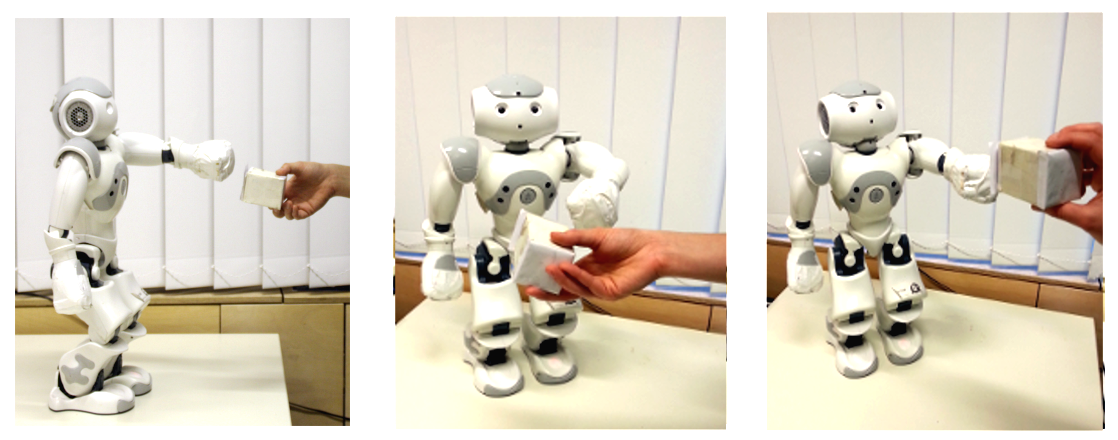
\includegraphics[height=3cm]{experiment_new.png}          
      \end{figure}
 
\end{frame}

%%%%%%%%%%%%%%%%%%%%%%%%%%%%%%%%%%%%%%%%%%%%%%%%%%%%%
%%%%%%%%%%%%%%%%%%%%%%%%%%%%%%%%%%%%%%%%%%%%%%%%%%%%%
\subsection{\scshape Results}
\begin{frame}{Hand trajectories}
\begin{itemize}
      \item Comparison of hand trajectories predicted by the two models for the horizontal dimension (cca. 1 sec)
      \begin{figure}[ht]     
      \epsfig{file=hand_trajectory.eps, height=5cm}     
      \end{figure}

\end{itemize}
\end{frame}

%%%%%%%%%%%%%%%%%%%%%%%%%%%%%%%%%%%%%%%%%%%%%%%%%%%%%%
%%%%%%%%%%%%%%%%%%%%%%%%%%%%%%%%%%%%%%%%%%%%%%%%%%%%%%
\section{\scshape Conclusion}
\begin{frame}[noframenumbering]
\Large Conclusion
\end{frame}


%%%%%%%%%%%%%%%%%%%%%%%%%%%%%%%%%%%%%%%%%%%%%%%%%%%%%
%%%%%%%%%%%%%%%%%%%%%%%%%%%%%%%%%%%%%%%%%%%%%%%%%%%%%
\subsection{\scshape Conclusion}
\begin{frame}{Conclusion}

\begin{itemize}	
	\item The proposed SOM-based model exhibits pointing when implemented on a humanoid robot
	  \begin{itemize}
	   \item Supports the hypothesis that pointing emerges from grasping \cite{Kaplan2006}
	  \end{itemize}
	\item Better pointing precision achieved with more neurons
	\item Interesting directions for the future research: spiking neurons and more complex learning rules (e.g. STDP)
\end{itemize}
\end{frame}

%%%%%%%%%%%%%%%%%%%%%%%%%%%%%%%%%%%%%%%%%%%%%%%%%%%%%
\subsection{\scshape Conclusion}
\begin{frame}{Final words}
\begin{itemize}          
     \item More on this project:
     	\begin{itemize}
     		\item Talk to me :)
     		\item Read: \small{Kaji\'c, I., Schillaci, G., Bodiro\v{z}a, S., and Hafner, V. V. (2014). Learning hand-eye coordination for a humanoid robot using SOMs. In Proceedings of the 2014 ACM/IEEE International
Conference on Human-robot Interaction, HRI 14, pages 192 - 193, New York, NY, USA. ACM.}
	      \item Python source code online: \url{github.com/ikajic/cog-rob}
     	\end{itemize}
     \item More on these slides and the poster:
     \begin{itemize}
      \item Made in \LaTeX (open-source program)
      \item \LaTeX code for both available online: \url{github.com/ikajic/uni-templates}
      \item Open-source: Because sharing knowledge (for free) is important!
     \end{itemize}     
\end{itemize}
    
\end{frame}



\subsection{\scshape Conclusion}
\begin{frame}        
  \bibliographystyle{apalike}
  \bibliography{literatur.bib}
\end{frame}

\subsection{\scshape Conclusion}
\begin{frame}[noframenumbering]
\Large Appendix
\end{frame}


\appendix

%%%%%%%%%%%%%%%%%%%%%%%%%%%%%%%%%%%%%%%%%%%%%%%%%%%%%
%%%%%%%%%%%%%%%%%%%%%%%%%%%%%%%%%%%%%%%%%%%%%%%%%%%%%
\begin{frame}{Pointing precision}
\begin{itemize}
      \item The Euclidean distance between the object and the hand 
      \item A paired-samples t-test ($t(1400)=76.47$, $p<0.05$) showed a  significant difference between two the models
      \begin{table}[h]\footnotesize
      \label{lab:table}
      \begin{tabular}{|c|c|c|}
	\hline     
	  & Mean (mm) & Std. Dev. (mm) \\ \hline
	$5\times 5$ & $99.93$ & $32.10$ \\ \hline
	$15\times 15$ & $80.32$  & $33.41$ \\ \hline
      \end{tabular}
      \end{table}      
      
	%\item \small{$5 \times 5$ network ($Mean\ error=99.93mm$, $Std.\ Dev.=32.10$)}
	%\item \small{$15 \times 15$ network ($Mean\ error=80.32mm$, $Std.\ Dev.=33.41$) conditions; $t(1400)=76.47$, $p<0.05$}
\end{itemize}
\end{frame}

%%%%%%%%%%%%%%%%%%%%%%%%%%%%%%%%%%%%%%%%%%%%%%%%%%%%%
%%%%%%%%%%%%%%%%%%%%%%%%%%%%%%%%%%%%%%%%%%%%%%%%%%%%%
\begin{frame}{Hand trajectories}
\begin{itemize}
      \item Comparison of hand trajectories predicted by the two models for the vertical dimension 
      \begin{figure}
      \includegraphics[scale=0.4]{trajectory_y1.png}      
      \end{figure}

\end{itemize}
\end{frame}



%%%%%%%%%%%%%%%%%%%%%%%%%%%%%%%%%%%%%%%%%%%%%%%%%%%%%
%%%%%%%%%%%%%%%%%%%%%%%%%%%%%%%%%%%%%%%%%%%%%%%%%%%%%
\begin{frame}{Hand trajectories}
\begin{itemize}
      \item Comparison of hand trajectories predicted by the two models for the depth dimension 
      \begin{figure}
      \includegraphics[scale=0.4]{trajectory_z.png}      
      \end{figure}

\end{itemize}
\end{frame}

\begin{frame}{Random Body Babbling - Limitations}
\begin{itemize}       
      \item Does not assume any goal directed behaviour (but there's: goal babbling) 
      \item Inability to switch between exploration of new postures and exploitation of existing ones based on robot's learning interest
      \item There are more advanced exploration behaviours, but they were out of scope of this thesis	
\end{itemize}
\end{frame}


\begin{frame}{Embodied Cognition}
\begin{itemize}
      \item The idea that our cognition is influenced/shaped/determined by our experiences in the physical world
      \item "Thought is tightly constrained, and at the same time enabled by the body`` (Pfeifer and Bongard, 2007)
      \item "We propose that seeing is a way of acting. It
is a particular way of exploring the environment. Activity in internal representations does not generate the experience of seeing. '' (Regan and Noe, 2001)
      \item Perceptual experience very often incorporates anticipated embodied interaction

\end{itemize}
\end{frame}



\begin{frame}{SOMs are (not) Biologically Inspired}
\begin{itemize}       
      \item \emph{A Possible Embodiment of Self-Organization in a Neural Structure} (Section 3 in "Self-Organized Formation of Topologically Correct Feature Maps`` (Kohonen 1982)
      \item Two mechanisms:
      \begin{itemize}
        \item Formation of activity cluster (anatomical and physiological evidence)
	\item Adaptive change in input weights (limited synaptic resources)
      \end{itemize}

      \begin{figure}[t]
      \centering
      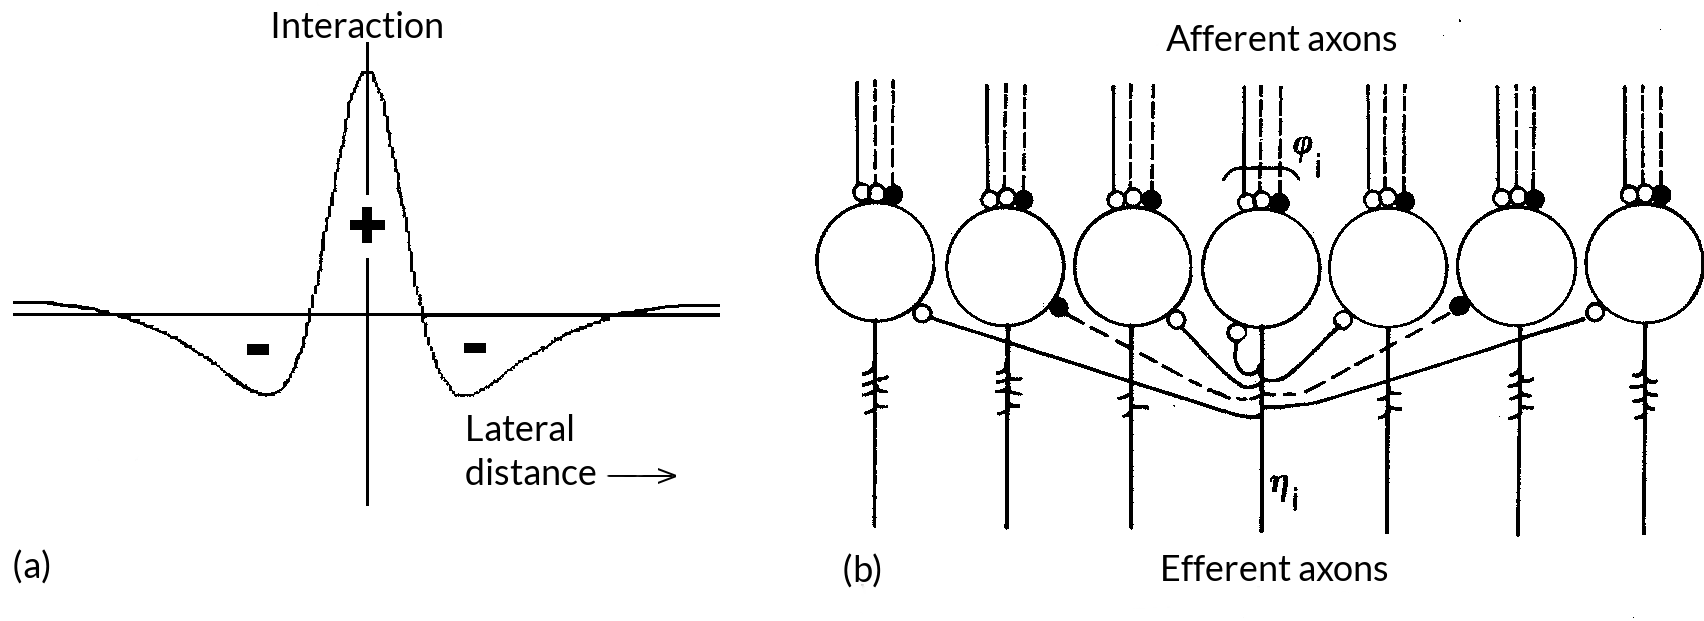
\includegraphics[scale=0.15]{soms_bio_hor.png}      
      \end{figure}

\end{itemize}
\end{frame}


\end{document}
